% **************************************************************************************************************
% A Classic Thesis Style
% An Homage to The Elements of Typographic Style
%
% Copyright (C) 2015 André Miede http://www.miede.de
%
% If you like the style then I would appreciate a postcard. My address 
% can be found in the file ClassicThesis.pdf. A collection of the 
% postcards I received so far is available online at 
% http://postcards.miede.de
%
% License:
% This program is free software; you can redistribute it and/or modify
% it under the terms of the GNU General Public License as published by
% the Free Software Foundation; either version 2 of the License, or
% (at your option) any later version.
%
% This program is distributed in the hope that it will be useful,
% but WITHOUT ANY WARRANTY; without even the implied warranty of
% MERCHANTABILITY or FITNESS FOR A PARTICULAR PURPOSE.  See the
% GNU General Public License for more details.
%
% You should have received a copy of the GNU General Public License
% along with this program; see the file COPYING.  If not, write to
% the Free Software Foundation, Inc., 59 Temple Place - Suite 330,
% Boston, MA 02111-1307, USA.
%
% **************************************************************************************************************
\documentclass[ twoside,openright,titlepage,numbers=noenddot,headinclude,%1headlines,% letterpaper a4paper
                footinclude=true,cleardoublepage=empty,abstractoff, % <--- obsolete, remove (todo)
                BCOR=5mm,paper=a4,fontsize=11pt,%11pt,a4paper,%
                ngerman,american,%
                ]{scrreprt}

%********************************************************************
% Note: Make all your adjustments in here
%*******************************************************
\input{thesis-config}

%********************************************************************
% Bibliographies
%*******************************************************
\addbibresource{bibliography.bib}

%********************************************************************
% Hyphenation
%*******************************************************
%\hyphenation{put special hyphenation here}

\begin{document}
\frenchspacing
\raggedbottom
\selectlanguage{american} % american ngerman
%\renewcommand*{\bibname}{new name}
%\setbibpreamble{}
\pagenumbering{roman}
\pagestyle{plain}
%********************************************************************
% Frontmatter
%*******************************************************
\listoftodos\cleardoublepage

\include{frontbackmatter/DirtyTitlepage}
\include{frontbackmatter/Titlepage}
\thispagestyle{empty}

\hfill

\vfill

\noindent\myName: \textit{\myTitle,} \mySubtitle, Master Thesis, %\myDegree, 
\textcopyright\ \myTime

\bigskip
%
\noindent\spacedlowsmallcaps{Supervisors}: \\
\myProf \\
%\myOtherProf \\ 
\mySupervisor \\
%
\medskip
%
\noindent \spacedlowsmallcaps{Location}: \\
University of Potsdam\\
Hasso-Plattner-Institut\\
Business Process Technology\\
Prof.-Dr.-Helmert-Str. 2-3\\
D-14482 Potsdam\\
%\myLocation
%
\medskip
%
\noindent\spacedlowsmallcaps{Time Frame}: February 21st -- August 21st, 2017 \\
%\myTime

\cleardoublepage%*******************************************************
% Abstract
%*******************************************************
%\renewcommand{\abstractname}{Abstract}
\pdfbookmark[1]{Abstract}{Abstract}
\begingroup
\let\clearpage\relax
\let\cleardoublepage\relax
\let\cleardoublepage\relax

\chapter*{Abstract}
Business Processes have become an essential tool in organizing, documenting and executing company workflows while Event Processing can be used as a powerful tool to increase their flexibility especially in destributed scenarios. 
The publish-subscribe paradigm is commonly used when communicating with complex event processing platforms, nevertheless prominent process modelling notations do not specify how to handle event subscription.

At the example of BPMN 2.0, the first part of this work illustrates the need for a flexible usage of event subscription in process models and derives new requirements for process modelling notations. An assessment of the coverage of these requirements in BPMN 2.0 is presented and shortcomings are pointed out.

Based on the identified requirements, this work presents a new concept for handling event subscription in business process management solutions, predominantly built on the notion of event buffers. The concept includes an extension to the BPMN meta model, specifies the semantics and API of a new event buffering module and describes the changes necessary to the behaviour of the process engine.

For evaluation purposes, the concept has been implemented as a reusable Camunda Process Engine Plugin that interacts with the academic Complex Event Processing Platform UNICORN.


\vfill

\begin{otherlanguage}{ngerman}
\pdfbookmark[1]{Zusammenfassung}{Zusammenfassung}
\chapter*{Zusammenfassung}
Kurze Zusammenfassung des Inhaltes in deutscher Sprache\dots 
\end{otherlanguage}

\endgroup			

\vfill
\pagestyle{scrheadings}
\cleardoublepage%*******************************************************
% Table of Contents
%*******************************************************
%\phantomsection
\refstepcounter{dummy}
\pdfbookmark[1]{\contentsname}{tableofcontents}
\setcounter{tocdepth}{2} % <-- 2 includes up to subsections in the ToC
\setcounter{secnumdepth}{3} % <-- 3 numbers up to subsubsections
\manualmark
\markboth{\spacedlowsmallcaps{\contentsname}}{\spacedlowsmallcaps{\contentsname}}
\tableofcontents 
\automark[section]{chapter}
\renewcommand{\chaptermark}[1]{\markboth{\spacedlowsmallcaps{#1}}{\spacedlowsmallcaps{#1}}}
\renewcommand{\sectionmark}[1]{\markright{\thesection\enspace\spacedlowsmallcaps{#1}}}
%*******************************************************
% List of Figures and of the Tables
%*******************************************************
\clearpage

\begingroup 
    \let\clearpage\relax
    \let\cleardoublepage\relax
    \let\cleardoublepage\relax
    %*******************************************************
    % List of Figures
    %*******************************************************    
    %\phantomsection 
    \refstepcounter{dummy}
    %\addcontentsline{toc}{chapter}{\listfigurename}
    \pdfbookmark[1]{\listfigurename}{lof}
    \listoffigures

    \vspace{8ex}

    %*******************************************************
    % List of Tables
    %*******************************************************
    %\phantomsection 
    \refstepcounter{dummy}
    %\addcontentsline{toc}{chapter}{\listtablename}
    \pdfbookmark[1]{\listtablename}{lot}
    \listoftables
        
    \vspace{8ex}
%   \newpage
    
    %*******************************************************
    % List of Listings
    %*******************************************************      
      %\phantomsection 
    \refstepcounter{dummy}
    %\addcontentsline{toc}{chapter}{\lstlistlistingname}
    \pdfbookmark[1]{\lstlistlistingname}{lol}
    \lstlistoflistings 

    \vspace{8ex}
       
    %*******************************************************
    % Acronyms
    %*******************************************************
    %\phantomsection 
    \refstepcounter{dummy}
    \pdfbookmark[1]{Acronyms}{acronyms}
    \markboth{\spacedlowsmallcaps{Acronyms}}{\spacedlowsmallcaps{Acronyms}}
    \chapter*{Acronyms}
    \begin{acronym}[UMLX]
        \acro{API}{Application Programming Interface}
        \acro{BPM}{Business Process Management}
        \acro{BPMN}{Business Process Model and Notation}
        \acro{CEP}{Complex Event Processing}
        \acro{EdBPM}{Event-driven Business Process Management}
        \acro{EPL}{Event Processing Language}
        \acro{JVM}{Java Virtual Machine}
        \acro{HTTP}{Hypertext Transfer Protocol}
        \acro{PEP}{Process Engine Plugin}
        \acro{REST}{Respresentational State Transfer}
        \acro{SQL}{Structured Query Language}
        \acro{UML}{Unified Modeling Language}
        \acro{XML}{Extensible Markup Language}
    \end{acronym}                     
\endgroup

%********************************************************************
% Mainmatter
%*******************************************************
\cleardoublepage\pagenumbering{arabic}
%\setcounter{page}{90}
% use \cleardoublepage here to avoid problems with pdfbookmark
\cleardoublepage
%\ctparttext{You can put some informational part preamble text here.}
%\part{Some Kind of Manual}
%************************************************
\chapter{Introduction}
%************************************************

Given the increasing competition on the global market place, companies are seeking to improve their products while reducing costs.
In many areas, \ac{BPM} has been chosen as one of the tools to help stay competitive.
Especially large enterprises, but also small to medium businesses formalize their work-flows in business process models to allow their automatized execution and management, archiving and documentation.

% maybe a little more on BPM?

With Business Process Technology in constant progression, the opportunities that the field has to offer are ever growing.
Since the recent years, many efforts have been dedicated towards bringing together business processes and \ac{CEP}.
By the help of event processing systems, companies are trying to get a hold of the exponentially growing amounts of data that occur in today's IT~environment.
Event Engines are designed to process thousands of events each second while supporting the integration of multiple event types and sources to derive new information.
%Therefor, incoming data is evaluated according to query expressions, themselves producing new, enhanced events.% by projection, filtering, aggregating or joining.
By having conglomerated information available almost in real-time, companies can react quickly on complex situations within their organization or anywhere on the world.
The connection of events and business processes has developed into an own discipline, \acl{EdBPM}, which is performed from two perspectives.
%- 2 variants of doing edbpm
%https://www.researchgate.net/profile/Oliver_Mueller5/publication/241635758_Extending_BPMN_for_Business_Activity_Monitoring/links/0deec52d00ef9276c9000000.pdf
%(BAM) refers to the observation, analysis, and presentation of real-time information about business activities across systems’ and companies’ borders.
During execution, business processes can take the role of an event producer and publish information about their status, errors or incidents. 
Processed through complex event processing, this information can be utilized for business activity monitoring which aims at providing timeliness and effectiveness of operational business processes.
In a second field of research, processes consume events so that the projected work-flow can be influenced and controlled.
By that means, events heavily increase the capabilities and flexibility in process flows. They can enable intra-organizational communication between processes or business departments, but also allow to respond to external situations within seconds and milliseconds.

The \ac{BPMN}, the most prominent industry standard for representing business processes,% both visually and through a textual model, 
natively supports the use of events in numerous fashions. Event-related elements are a main building block of the modeling language and can, for instance, be used for instantiating processes, communicating between process participants or to support decisions.
Thereby, event-driven process control combines the advantages of \acl{BPM} and Complex Event Processing.


\section{Motivation}

An interaction with a Complex Event Processing platform generally follows the publish-subscribe paradigm: The event consumer contacts the platform and issues a subscription to a specific subset of available events.
The event producer, for example a vehicle providing its current GPS location, publishes information to the event processing platform, which is then forwarded to every consumer that had subscribed.
As event processing has become an essential part of \ac{BPM}, there is a need for the available modeling frameworks to consider these interaction patterns.

This work investigates the aspect at the example of the \ac{BPMN}, where \textit{Intermediate Events} enable event-based process control between the start and the end of a process. %and hence facilitate the consumption of complex events. %reception of external message events.
However, the BPMN specification does not specifically consider the publish-subscribe work-flow and consequently provides only limited capabilities to represent event subscription and un-subscription operations in business process models.
From the execution semantics of intermediate events, the common interpretation is that the subscription to an event source implicitly happens when an event is enabled, the un-subscription on termination of the element~(see~\cite{} re-eval, mandal, earlier paper).
- mandal add the idea of issuing subscriptions explicitly through a customized service task.
%- while other work on the use of complex events does not mention subscription and un-subscription at all
% > probably assuming that a subscription is already active
%- there is research on including the subscription query in the model, but the subscription time is not further defined
Given that the subscription to an event must take place strictly before consumption, the time to listen to an event is limited to only a segment of the process execution.
Naturally, in event processing, a large number of participants can be involved to cause a complex event. This high level of distribution and the inclusion of external sources implies that the time of event occurrence cannot be entirely controlled.

As defined in the BPMN specification, an intermediate catch event will wait for the associated event to occur. In case the event does not occur or only after a significant amount of time, this behavior leads to a delay or even a complete halt of the process execution. %reduce process efficiency
While some process designs require just these semantics, in others they cause an unnecessary reduction of efficiency or fault.%the variable time of event occurrence
\todo[inline]{short example, maybe harvesting?}
This behavior is further illustrated by the help of two example scenarios in \autoref{ch:motivatingexamples}.

An earlier subscription to an event source would increase the timespan in that events can be received and thus reduce the probability of missing events.
This motivates the investigation of mechanisms to more flexibly incorporate subscribe operations in business processes.
% also definition of subscription stuff in general, because there is no standard.

%The ability to influence the event subscription time more flexibly 


%- to ensure the efficient use of events in processes, a more flexible use of subscription is necessary

%- that implies the additional need for buffers


%This work investigates the consequences of this lack of specification and provides a design and implementation to overcome the identified shortcomings.



\section{Contribution}
Working towards a more flexible use of event subscription in business processes...

> Maybe include structure

(0) reviewing the problem from different perspectives, deriving requirements
(1) assessment of the capabilities of standard bpmn
(2) Proposition of a BPMN extension for flexible event subscription, its advantages
(3) derived requirements to process engines and CEP platforms
(4) A reference implementation using Camunda and UNICORN


\section{Structure}
\todo[inline]{write}

\cleardoublepage%************************************************
\chapter{Background on Event-Driven Business Process Management}\label{ch:background}
%************************************************

\section{Business Process Management}
With its origins dating back to the process orientation trend of the 1990s, \ac{BPM} has meanwhile become a mainstream tool to support organizations.
It had been noted, that company workflows can essentially be broken down into activities that are executed in a coordinated manner by one or more parties.
A certain group of activities thereby form a process which is executed within an organization.
More precisely, \citeauthor{weske:bpm-book} \cite{weske:bpm-book} defines a single \emph{business process} as follows:

\begin{description}
	\item[Definition 1 (Business Process):]
	A \emph{business process} consists of a set of activities that are performed in coordination to realize a business goal. Each business process is enacted by a single organization, but it may interact with processes performed by other organizations. \cite[p.~5]{weske:bpm-book}
\end{description}

\noindent The term \emph{Business process management} describes the techniques available to develop and support processes throughout their life-cycle.
It is grounded in the use of explicit process representations which ultimately allow the exchange, analysis and reproduction of the workflows.
This process specification is referred to as the \emph{business process model}, composed of activities and the rules that are necessary to coordinate their execution. When a process is performed according to its model, the single execution is called \textit{process instance}.
Based on a process model, the number of possible instances is theoretically infinite.

\begin{description}
	\item[Definition 2 (Business Process Model):]
	A \emph{business process model} consists of a set of activity models and execution constraints between them. A \emph{business process instance} represents a concrete case in the operational business of a company, consisting of activity instances.
	\cite[p.~7]{weske:bpm-book}
\end{description}

While traditionally activities where executed manually by company staff following the written process specifications, computer systems are used today to drive the execution and enforcement of business processes and organizational rules.
The generic software systems utilized for that purpose are introduced in the following \autoref{ch:bg:bpms}.

\todo[inline]{not only one source}

\subsection{Business Process Management Systems}\label{ch:bg:bpms}
The implementation of business processes has developed from a manual execution guided by business rules to a fully automatized execution in a specialized IT environment.
One of the main reasons for \acs{BPM}'s growing popularity is that in today's fast-paced economy, a large part of the business activity is either supported by computers or even carried out autonomously by them.
The specialized software systems that are utilized to support the enactment of business processes are referred to as \emph{business process management systems}.

\paragraph{Business Process Lifecycle}

- the investigations undertaken in this work target the Design \& Analysis phase

\paragraph{Process Management Reference Architecture}
A typical IT infrastructure for running and maintaining business processes comprises the following building blocks:



\missingfigure{bpm it infrastructure: modeling tool, model repository, users, process engine, external service providers}

talk about their basic architecture, process engine
+ phases: deployment, enactment, un-deployment

\paragraph{The Camunda Business Process Engine}\label{ch:bg:camunda}
- there are many process engines
- camunda is open source and popular and modern and actively developed
- the camunda project and its current state
- parts of the camunda software
- some outstanding features
- why do I mention this?


\subsection{Business Process Model and Notation}
- different modeling notations are available, each serving a different purpose / specialization
> BPM Systems require an explicit representation, but support different modeling languages. A more recent industry standard is . .. ,currently available in version 2.0, published in ...
- modeling notation, focus on ..., 2.0, Object Management Group
- main elements:
-> briefly explain
- events: why? how?
- Message
- choreographies

\missingfigure{Sample BPMN business process}

- explain what happens in that process

\section{Complex Event Processing}
- what does it do
- how does it generally work
-> stream processing and | input > processing > output |
- Event queries: Esper
- event producer, consumer, subscription
-> pub/sub; temporal order sub > occur > unsub

\missingfigure{pub/sub workflow}

\section{Events in Business Processes}
- interplay BPT to CEP platforms, 
> sub in BPMN should rather be 'Problem Statement' somehow
- putting cep queries into bpmn models => heiko's thesis or other related work?
- how can events be used
- exercise through one example




\cleardoublepage%************************************************
\chapter{Problem Statement}\label{ch:problemstatement}
%************************************************

Event subscription is an essential part of event-driven architectures and must consequently be considered when using events in business processes.
While the use of external events is an active topic in research, most approaches only briefly discuss the subscription mechanism and use the \acs{BPMN}~semantics for orientation.
\todo[inline]{ref}
Though event subscription is not directly addressed in the BPMN~specification, the descriptions on intermediate events state:

\paragraph{}
\textit{"For Intermediate Events, the handling consists of waiting for the Event to occur. Waiting starts when the
Intermediate Event is reached. Once the Event occurs, it is consumed."}~\cite{bpmnspec},~p.~440\newline

\noindent The usual interpretation of this excerpt is that the subscription to the event takes place as soon as the event gets enabled, the un-subscription when the event terminates.
\todo[inline]{I need to work with a precise lifecycle}
As pointed out by Mandal~et.~al.~\cite{mandal:2017}, these subscription semantics significantly limit the flexibility of using events in business processes and can cause undesired behavior and fault.
Due to the strict temporal order between event subscription, occurrence and un-subscription as required by the publish-subscribe paradigm, any events that occur before the enabling of the event element will be ignored by the process execution.
That reduces the timespan for events to occur to a potentially small part of the total execution time and means that crucial events might be missed.

In the following section, the problem is further illustrated at the example of two sample scenarios.
The observed situations then lead to the definition of \textit{Event Occurrence Scenarios} and the derivation of a set of requirements that must be fulfilled by a mechanism for flexible event subscription in business processes.

\section{Motivating Examples}\label{ch:motivatingexamples}
% some has been mentioned in the introduction
%illustrate the complexity

To allow a better understanding of the issue, event-driven use-cases from two different domains are presented in the following.
The cases are revealed through their standard BPMN representation.
It is illustrated, why the time of event subscription is of great importance which motivates to study the mechanics and implications of event subscription in business processes.

\paragraph{Delay of a logistics process}
The first example~(\autoref{fig:example-eurotunnel}) is taken from the logistics domain and shows a truck transport that has to cross the English Channel.
The truck driver receives the transport plan for his next tour from France to the UK. By default, the company crosses the Channel using the Eurotunnel, an underground train connection between London and Paris.

\begin{figure}[]
	\myfloatalign
	{\includegraphics[width=1\linewidth]{chapters/requirements/Eurotunnel-simplified.png}}
	\caption{BPMN Model of a Logistics Process using events for route~optimization~(Example 1.1)}
	\label{fig:example-eurotunnel}
\end{figure}

After loading the goods at the factory, the truck will head towards the check-in location of the Eurotunnel.
If everything runs on schedule, the truck crosses the channel on the train and then delivers the goods in Great Britain.
Alternatively, the process considers a route using the ferry from Calais~(FR) to Dover~(UK).
The Eurotunnel administration publishes delay information approximately every 30~minutes through an RSS feed on their website. While it mostly operates on schedule, delays ranging from 15~minutes to several hours occur regularly. It can happen that new information is not published for multiple hours.
Significant delay events (delay~>~30~minutes) are received through a boundary catching message event attached to the activity \textit{Drive to Eurotunnel Check-In}. The boundary event is interrupting, hence the activity is canceled if a delay occurs.
The transport continues towards the ferry terminal and crosses the English Channel over sea. After crossing the channel, the goods are delivered to the recipient.
\todo[inline]{show a cep query for that scenario to make it more precise}

As interpreted from the BPMN specification, the subscription to the boundary event is issued as soon as the related activity is enabled.
Given that events arrive every 30~minutes, there can be a gap of up to half an hour, before the first information becomes available.
In the worst cases, when data isn't published for several hours, this gap will be even bigger.
Let's consider a very busy weekday; A technical fault occurred in the tunnel earlier that day and the train runs 3 hours behind schedule.
The last information on the RSS feed was published at 2:35\,pm. At that time the truck driver is still in the process of loading goods, finishing the activity at 2:40\,pm.
Following the process definition, the driver now departs towards the Eurotunnel check-in.
The system publishes updated information at 3:15~pm, operations are still 2:30\,h behind schedule. The message gets received through the process and the truck driver takes the alternative route to the ferry, but only after heading to the Eurotunnel for 35~minutes. The late change of plans causes an unnecessary delay to the shipment.

\begin{figure}[]
	\myfloatalign
	{\includegraphics[width=1\linewidth]{chapters/requirements/Eurotunnel_part2.png}}
	\caption{Transport via English Channel that is timed to a delivery~slot~(Example~1.2)}
	\label{fig:example-eurotunnel-part2}
\end{figure}

\autoref{fig:example-eurotunnel-part2} is an extension of the the transport process.
In logistics, it is common that a delivery cannot be accepted at an arbitrary time. Instead, the receiving party assigns delivery windows to the transport company.
The transport must arrive during the given time window, otherwise the delivery cannot be completed.
After crossing the English Channel, the process model shows the catching of a message event containing the desired final arrival time at the factory. There is an agreement with the factory, that the delivery slots will be approved 2~hours before the expected arrival.
If the current ETA of the transport is greater or equal to the arrival time, the driver will head to the drop-off point immediately. If the transport is ahead of schedule, the driver will have to delay the delivery to match the time window.

The presented process model illustrates another complexity of using events in processes. Again, the listening to the announcement of a delivery window will start when the event element is enabled, in this case after crossing the English Channel. 
Until an event has been received, the process will not continue. 
Much worse: if the receiving party sends out the arrival time information too early, \ie~while the truck is crossing the channel, the event is missed. If it is not issued again, the process cannot receive a message and will get stuck indefinitely waiting to catch the event.

Neither of the two presented catch events allow for an efficient and reliable execution of the process. They can cause unnecessary delays and even blocking of the process execution.

\todo[inline]{Consider more possible event occurrence times to prepare for the next chapter}

\paragraph{Up-to-date shipping information for an order}
\begin{figure}[]
	\myfloatalign
	{\includegraphics[width=1\linewidth]{chapters/requirements/Retail-Order.png}}
	\caption{Model of a retail order management process (Example 2)}
	\label{fig:example-order}
\end{figure}

A~similar situation can be observed in the order-management process depicted in \autoref{fig:example-order}.
It describes the interaction between customer and seller in a traditional distance retail scenario: After browsing the product catalog, the customer requests a quote for the articles he or she is willing to buy.
The retailer makes an offer including an approximation of the expected shipment date and sends it to the customer. That quote is then either accepted or not and the payment is issued if necessary.
Once the retailer is informed about the placement of the order, the products are packed and shipped as soon as possible.
For articles that are not currently in stock, the retailer must await the shipment from the factory. If any of the factory-shipments is delayed, the retailer cannot ship in time and will announce a delayed shipment date to the customer.
This situation is modeled through a non-interrupting boundary event attached to the \textit{Prepare Shipping} activity, which triggers the sending of the updated shipment date to the customer.

The process shows a number of similarities, but also differences in terms of event-use when compared to the logistics process in Example~1.
At first we look at the three intermediate catch events, \textit{Quote~received}, \textit{Order~canceled} and \textit{Order~placed}.
In each of the cases, the event to be caught is the direct response to a message that was sent right before. While the process will also enter a waiting state until the response arrives, that waiting is not to be interpreted as an unnecessary delay to the process execution.
Other than in Example~1.2\,(\autoref{fig:example-eurotunnel-part2}), there is nothing useful to do before the response is received.
It is furthermore worth noting that the response messages cannot be missed, because the message catch event immediately follows the message send event.

A different situation holds for the boundary event \textit{Shipment Delay}.
While the subscription to a Eurotunnel event can be issued at any time, it does not depend on any process data, the shipment delay has to be observed for each product that is part of the order. A subscription can therefor not be executed before the activity \textit{Prepare~Quote} has terminated. \todo[inline]{show a cep query for that scenario to make it more precise}
Conforming to the definition of the process, the system will listen to shipment delays once the activity \textit{Prepare~Shipping} is enabled and therefor much later than possible.
Any events that occur after the completion of \textit{Prepare~Quote} but before \textit{Prepare~Shipping}, cannot be considered in the process execution and the customer will not be informed about a possible late shipment. That will, for instance, concern events that occur while the customer makes the decision about accepting or canceling the order.

% The first of these three follows the \textit{Send/Receive} Service Interaction Pattern. \todo[inline]{missingref}
% Two parties interact 

\medskip \noindent 
The two presented examples have illustrated the complexity of using events in business processes, especially when all possible event occurrence times are taken into consideration.
Differences have been pointed out as to how exactly the event is placed in the process, if it waits for a direct response to an earlier request or if the event occurrence is unrelated to the execution of that very process.
Motivated by this complexity and the possible implications, it is the goal of this work to evaluate the capabilities of BPMN and to present a concept for the flexible handling of event subscription in business processes.


\section{Event Occurrence Scenarios}
Given the motivating examples, a generic set of \textit{Event Occurrence Scenarios} is defined in this section. 
Each of the scenarios represents a real-world situation and process implementations need to be capable of handling them to avoid negative effects.

\medskip \noindent
The dominant variable to consider is the event occurrence time.
According to the BPMN specification, it is possible to catch an event if it occurs after the event element is enabled. As shown before, it is often impossible to control occurrence time and events do occur outside of the listening time intervals.
An \ac{EOS} describes the time of event occurrence in relation to a specific step in process or engine execution.
The life-cycle of a process within a process engine is explained in \autoref{ch:bg:bpm} and taken as reference. It is assumed that the process and event engine are configured and running.W
An event is considered to always occur before or after a life-cycle step or in between two consecutive steps. 
Given the life cycle steps \textit{process deployment}, \textit{process instantiation} and \textit{event enabling}, the following occurrence scenarios are distinguished in this work:
% they have an implicit temporal order

\begin{aenumerate}
	\item[$EOS_{1}$] While the BPMN event element is enabled
	\item[$EOS_{2}$] The event does not occur
	\item[$EOS_{3}$] Between process instantiation and \\the enabling of the BPMN event
	\item[$EOS_{4}$] Between process deployment and \\process instantiation
	\item[$EOS_{5}$] Before process deployment
\end{aenumerate}\label{def:occurrence-times}
% they are ordered this way to be in line with the assessment chapter

\begin{figure}[]
	\myfloatalign
	{\includegraphics[width=1\linewidth]{chapters/requirements/timeline-event-occurrence.png}}
	\caption{Possible event occurrence times in relation to a process execution life cycle}
	\label{fig:occurrence-timeline}
\end{figure}\todo[inline]{improve figure: include EOS notions, save space, ?}

An overview of the EOSs and the related life-cycle steps is provided in \autoref{fig:occurrence-timeline}, which uses a time-line to illustrate the possible event occurrence times.
The model deliberately excludes event occurrences after termination of the event element, because that would presume that there is no more interest in the event as the execution flow continued on another branch. Otherwise, the process will remain in waiting state until the event occurs.

\todo[inline]{add a back reference to the examples. In example XY, events can occur before... whereas in example...}

As introduced in \autoref{ch:bg:cep}, there is a strict temporal order between event subscription, reception and un-subscription.
To catch an event that occurs as described in any of the EOSs, the related subscription operation has to be executed before the start of the time interval associated with the EOS.
On that basis, the latest possible event subscription time can be derived from each event occurrence scenario and is as follows:
\textit{before process deployment}~($EOS_{5}$), \textit{during process deployment}~($EOS_{4}$), \textit{at process instantiation}~($EOS_{3}$) and when the \textit{BPMN event element is enabled}~($EOS_{1}$).

It is important to highlight that the subscription to an event source can depend on additional context information or process data, which can be a significant limitation to the possible subscription time.
That situation is illustrated in \textit{Example~2}~(\autoref{fig:example-order}), where the subscription to the shipment delay information cannot be executed before the \textit{Prepare~Quote} activity is completed.
More generally put, a \textit{subscription~dependency} is defined as follows:

\begin{description}
	\item[Subscription Dependency]
	The subscription operation is \textit{dependent}, if any of its parameters, for instance the event query, contains a variable value that has to be determined at the time of subscription.
	The value might reference a piece of information from the process instance context, an engine-wide piece of data or external information.
	In case of a dependence, the subscription cannot be issued before the associated information is available.
\end{description}

If a subscription dependency resolves before the process execution reaches the event element, it should still be possible to flexibly chose the subscription time in the process.
For that reason, in addition to the four subscription-time options presented earlier, an additional option \textit{at any time during process execution} must be available.


\section{Requirements Definition}
The previous sections have exemplified how the execution semantic offered by the BPMN specification limits users in the use of events in business processes. Now these shortcomings are formalized into an additional set of requirements that must be met by a process execution environment to enable event handling in the extended set of event occurrence scenarios.
The formal requirements will later be used to evaluate the capabilities of current Process Management Solutions~(\autoref{ch:assessment}) and to develop a new concept to handling event subscription in business processes~(\autoref{ch:flexibleeventsubscription}).

\paragraph{R1: Flexible Event Subscription Time}

\begin{description}
	\item[R1.1 Explicitness:] 
	For each event that is used in a business process, it must be possible to derive the time of event subscription from the process model. The time of subscription may either be explicitly stated or defined implicitly.
	\item[R1.2 Flexibility:] 
	The time of subscription can be influenced to catch events according to any of the event occurrence scenarios O1, O2, O3, O4. In other words, the process model defines the earliest acceptable time for an event occurrence to be considered in the process execution. The necessary options are \textit{since system start}, \textit{since process deployment}, \textit{since process instantiation}, from an arbitrary but \textit{explicit time during process execution}, or \textit{since enabling of the Event Process Element}.
\end{description}


\todo[inline]{limited by subscription dependencies}
\todo[inline]{change the options back to the times of subscription. Mention that the subscription is necessary before the time of event occurrence, but too early subscription is also a problem.}
\todo[inline]{target only intermediate events. (limitation, although it also makes the most sense.)}

\paragraph{R2: Automatic Subscription Handling}

\begin{description}
	\item[R2.1 Subscription:] 
	The subscription to event sources is handled implicitly by the process execution environment as defined by the process model.
	\item[R2.2 Removal of Subscription:] 
	The removal of a subscription from the system is handled automatically as soon as a subscription becomes unnecessary.
\end{description}


\begin{description}
	\item[R3 Event Buffering:]
	To make all events since the subscription time available during process execution, matching events need to be stored temporarily.
\end{description}

\todo[inline]{buffer policies?}
\todo[inline]{variables and subscription dependencies}

\medskip \noindent
\todo[inline]{write connecting paragraph}
The remainder of this work will further analyze the capabilities of BPMN to express event-usage scenarios and propose solutions to the mentioned problems...

\cleardoublepage%************************************************
\chapter{Assessment of current Business Process Management Solutions}\label{ch:assessment}
%************************************************

The lack of flexibility in handling event subscription in business processes has been outlined in the previous chapters and a set of extended requirements to process management solutions have been presented.
In this section I take a closer look at the capabilities of current solutions with regards to the event occurrence scenarios to get a better understanding of the issues that arise when working with event subscription in business processes.
The assessment will be carried out using BPMN and Camunda, a state-of-the art and widely adopted business process engine.
The main goal is to identify and illustrate the shortcomings of the current process technology stack. These shortcomings will be referenced in addition to the presented requirements to develop a more refined subscription handling model in the following chapter. \todo[inline]{"subscription handling model"?}

\todo[inline]{which functionality should be evaluated exactly?: all occurrence scenarios, but no buffer policies. The buffer will always store the last version of the event and also deliver that version.}

\section{BPMN Models in presence of the Event Occurrence Scenarios}
Chapter X has revealed that processes can run into deadlocks if events do not occur at the right time \todo[inline]{.}
\begin{figure}[]
	\myfloatalign
	{\includegraphics[width=1\linewidth]{chapters/assessment/process-with-intermediate-event.png}}
	\caption{Abstract Process using an Intermediate Catch Event}\label{fig:abstract-process-with-event}
\end{figure}

\autoref{fig:abstract-process-with-event} shows a generalized process that uses an Intermediate Catch Event just before process termination.
In this section I first describe for each Event Occurrence Scenario how this simple event implementation behaves in presence of the given scenario. I then evaluate if it is feasible to create a BPMN model that is free from deadlock in these situations. 

\paragraph{Scenario O1: The event occurs after the enabling of the BPMN event}
\begin{figure}[]
	\myfloatalign
	{\includegraphics[width=1\linewidth]{chapters/assessment/standard-intermediate-event.png}}
	\caption{Standard Intermediate Catch Event}\label{fig:excerpt-standard-event}
\end{figure}

The first scenario represents the most simple case, that is also natively supported by the BPMN 2.0 specification. When the event occurs after the Event element has been enabled, the event will be received and the process can proceed normally. The use of a standard Intermediate Catch Event does suffice to cover this situation.

\paragraph{Scenario O2: The event does not occur}
\begin{figure}[]
	\myfloatalign
	{\includegraphics[width=1\linewidth]{chapters/assessment/parallel-timer-event.png}}
	\caption{Intermediate Event with a parallel Timer Event}\label{fig:excerpt-event-with-timer}
\end{figure}

In certain situations an event might not occur at all. Given a basic event implementation like in \autoref{fig:abstract-process-with-event}, the process flow will get to a halt once it reaches the Intermediate Catch Event and will not be able to proceed. While, depending on the process design, this might be the desired behavior, in many situations this is not acceptable.

Let's consider a process that is supposed to wait for approval for a certain amount of time and trigger an additional request if the approval has not been issued before the deadline. \autoref{fig:excerpt-event-with-timer} shows how this behavior can be implemented using an Event-based Gateway which puts a Timer Event in parallel to the Intermediate Catch Event. This extension will make sure that a process does not run into a deadlock state if the expected event does not occur.

\todo[inline]{I mention an example, but that example is not exactly illustrated in the process}
\todo[inline]{according to the spec: what exactly will happen to the active catch event once the timer fires?}


\paragraph{Scenario O3: Occurrence between Process instantiation and the enabling of the BPMN event}
\begin{figure}[]
	\myfloatalign
	{\includegraphics[width=1\linewidth]{chapters/assessment/parallel-gateway-early-subscription.png}}
	\caption{Event Element in parallel process flow}\label{fig:excerpt-parallel-gateway-event}
\end{figure}

In case the event occurs during process execution, but before the BPMN event element is enabled and thus listening for events, the occurrence will not be considered in the execution. The process will get stuck at the Event Process Element as if the event did not happen at all.
To avoid a deadlock in this scenario, a solution is to execute the Intermediate Catch Event in parallel to the rest of the process flow using a Parallel Gateway. This is illustrated in \autoref{fig:excerpt-parallel-gateway-event}. The time of subscription to the event can be controlled by the position of the parallel split: To implement an event subscription right after process instantiation, the Parallel Gateway has to be the first element after the Start Event (that means \textit{Part~1} in the illustration is empty). To implement event subscription at a specific point during process execution, part of the process can execute before reaching the Parallel Gateway. In \autoref{fig:excerpt-parallel-gateway-event}, the event may occur at any time during the execution of the collapsed sub-process \textit{Part~2}. 

\paragraph{Scenarios O4 and O5: Before Process Instantiation}
\begin{figure}[]
	\myfloatalign
	{\includegraphics[width=1\linewidth]{chapters/assessment/aux-buffer-process.png}}
	\caption{Event Buffering through an auxiliary Buffering Process}\label{fig:aux-buffering-process}
\end{figure}

Any Events that happen before process instantiation will not be considered in a standard Intermediate Catch Event. That applies to both scenarios, the occurrence between deployment and instantiation (\textit{O4}) and an occurrence time before the deployment of the process in the Process Engine (\textit{O5}).

To create a Process Model that allows to catch an event before the process instance exists, three new elements are introduced: (1) An additional \textit{Auxiliary Buffering Process} that can catch an incoming event, (2) an \textit{Event~Buffer}, a temporary data-store that keeps event data until required by the \textit{Original~Process}, (3) an \textit{Auxiliary Event Delivery Process}, that retrieves events from the buffer and makes them available to the \textit{Original~Process}.
\autoref{fig:aux-buffering-process} reveals the interaction of the \textit{Original Process}, the two auxiliary processes and the data-store. To start listening for an event, the \textit{Auxiliary Buffering Process} has to be instantiated through the a message start event containing the information necessary for the event subscription. The process starts listening for the event and writes the received event to the temporary data-store. 
The given process design is able to handle multiple event occurrences, because the receiving activity is looping. The buffering process terminates once the \textit{Unsubscribe} event is received.

\todo[inline]{how should the ABP be started? manually?}

The \textit{Original Process} can be started any time after the buffering process. In \autoref{fig:aux-buffering-process}, the Intermediate Catch Event has been explicitly split into three events: An initial Send Event to request events, a Catch Event to receive and a final Send Event to signal that no events shall be received anymore.
The initial Send Event instantiates the \textit{Auxiliary Event Delivery Process}, which tries to read from the Event Buffer and deliver the event to the Original Process. Once there is data available in the buffer, it is sent by the sending activity. The central looping activity will retry reading from the buffer until data becomes available and will only be terminated once the \textit{Stop}-event occurs. 
The Original Process can receive the event using a standard Intermediate Catch Event even when the event occurs before the instantiation of \textit{Original Process}, so it handles scenario \textit{O4}. 
Moreover the \textit{Auxiliary Buffering Process} is not bound to a specific event, it works generically with any event information that is passed on to it. For that reason it is also not bound to a specific process deployment and can buffer events even before a process has been deployed, so it handles scenario \textit{O5}.
Given that the buffering process can alternatively be started using an explicit Message Send Event during process execution and the process does not stop listening until the Original Process has received the event, scenarios \textit{O1} and \textit{O3} are also supported.

\todo[inline]{what exactly is passed around|how many instances of each process|overwrite or append to buffer|this is only one solution to do this, one that requires minimal changes in the original process}

\section{Implemention of Early Event Subscription using standard Camunda}
The previous chapter has shown that that it is possible to create BPMN models to match each of the Event Occurrence Scenarios, though for the scenarios \textit{O4} and \textit{O5} the solution becomes increasingly complex.
In the next step I investigate the capabilities of Camunda, a modern and actively developed Business Process Engine that is available under an open source license.
Camunda shall be used without any code customization, that means as offered on the website.
The solution presented for the last two scenarios has proven capable enough to handle all Event Occurrence Scenarios, therefor the goal is to implement this solution. It will be necessary to create the two auxiliary processes and a data-store in addition to the original process that makes use of the event buffering.

Two generic sample processes have been modeled for demonstration purposes. \autoref{fig:camunda-example-o3} shows a simple process with an explicit subscription activity to represent the listening to the event after process instantiation but before reaching the Catch Event (Scenario \textit{O3}). It follows a sample activity that takes 15 seconds (implemented using a \textit{Script Task}), the Intermediate Catch Event and another Script Task that displays the content of the received message.
The example for scenarios \textit{O4} and \textit{O5} (see \autoref{fig:camunda-example-o4-o5}) comprises the following elements: After the start event follows an Intermediate Catch Event, then an activity that prints the message of the event to console and last the Process End Event. Both figures show the processes as modeled in the Camunda Modeler.

\begin{figure}[]
	\myfloatalign
	{\includegraphics[width=1\linewidth]{chapters/assessment/example-o3.PNG}}
	\caption{Generic Example Process in Camunda for Occurrence Scenario \textit{O3}}\label{fig:camunda-example-o3}
\end{figure}

\begin{figure}[]
	\myfloatalign
	{\includegraphics[width=1\linewidth]{chapters/assessment/example-o4-o5.PNG}}
	\caption{Generic Example Process in Camunda for Occurrence Scenarios \textit{O4} and \textit{O5}}\label{fig:camunda-example-o4-o5}
\end{figure}

\paragraph{Auxiliary Buffering Process}
The task of this process is to subscribe to a CEP Platform using a provided event query and start listening for events. Any incoming event must be stored in a data-store (\textit{Event Buffer}).
UNICORN, an Esper-based academic event processing platform, will be used in this example.
A local MySQL database has been chosen for buffering the event data because it's freely available, quick to set up, offers standardized access via SQL queries and Java connectors and will persist data to the local harddrive by default. As UNICORN also requires an SQL database, the MySQL instance can be used in both cases.

\autoref{fig:camunda-aux-buffering-process} shows the final Buffering Process modeled in the Camunda Process Modeler. The process can be instantiated by issuing a \textit{Buffering Task} message. This message must contain three data fields: \textit{processDefinitionId}, to know which process definition the buffered messages belong to; \textit{messageName}, the name of the message event within the process; \textit{query}, the event query in the Esper Query Language.
Camunda will make the message data automatically available in the process instance as process variables, so they can be used during the execution of the Buffering Process.
After instantiation, the process reaches the activity \textit{Subscribe to Event Source}, a \textit{Java Service Task} that executes a HTTP call to the UNICORN platform. That call registers the event query in UNICORN. \todo[inline]{it tells unicorn its own instanceId, so that unicorn can correlate events to that exact instance}
Afterwards, the process reaches the receiving activity \textit{Wait for unsubscribe event} that will terminate the process as soon as the \textit{Unsubscribe} event has been received.
As long as this activity is active, events can be received through the attached Non-Interrupting Boundary Event. Incoming events have a field \textit{eventBody}, which contains the event information and becomes available through a process variable with the same name. \todo[inline]{does the message from UC have a field 'eventBody'?}
The boundary event triggers the service task \textit{Write eventBody to datastore}, which takes the data from the process variable and writes it to the MySQL Database Instance (\textit{Global Event Buffer}).

\begin{figure}[]
	\myfloatalign
	{\includegraphics[width=1\linewidth]{chapters/assessment/buffering-process.PNG}}
	\caption{Auxiliary Buffering Process in the Camunda Modeler}\label{fig:camunda-aux-buffering-process}
\end{figure}

\paragraph{Auxiliary Event Delivery Process}
The delivery process (see \autoref{fig:camunda-aux-event-delivery}) reads the latest data from the buffer and sends it to the process instance. It can be started with a message that contains the \textit{processInstanceId} and the \textit{processDefinitionId} of the requesting process and the \textit{messageName} of the Message Event that is requested from the buffer.
A \textit{Delay} Timer Event has been inserted to make sure that the receiving process is already in listening state, the execution happens asynchronously.
It follows the service task \textit{Retrieve event from buffer}, which executes Java code to read from the MySQL Database \textit{Event Buffer} and store the event information in a process variable named \textit{eventMessage}.
The content of that process variable is sent to the \textit{Original Process} in the Send Event, afterwards the execution is finished.


\begin{figure}[]
	\myfloatalign
	{\includegraphics[width=1\linewidth]{chapters/assessment/buffer-delivery-process.PNG}}
	\caption{Auxiliary Event Delivery Process in Camunda Modeler}\label{fig:camunda-aux-event-delivery}
\end{figure}


\paragraph{Interaction of the Processes}
In this implementation of flexible event subscription, the action of subscribing to the event source and the reception of events in the Original Process are splitted into two separate parts, each supported by an auxiliary process.
To initiate the subscription at the event source, the Auxiliary Event Buffering process has to be started.
For scenario \textit{O3}, this happens through an extra activity (\textit{Trigger Buffering Process}) during process execution, so that events after process instantiation are received by the Buffering Process.
In scenarios \textit{O4} and \textit{O5}, the subscription and thus the instantiation of the Buffering Process must happen before the instantiation of the Target Process. As there is no such mechanism in the standard Camunda Process Engine, the Buffering Process must be started by hand, providing the \textit{processDefinitionId}, the \textit{messageName} and the \textit{eventQuery}.

Now that the \textit{Buffering Process} is running, any events matching the query will be stored to the buffer.
When the Target Process reaches the Catch Event, a request for buffered events is sent as a message to trigger the \textit{Auxiliary Event Delivery Process}.
This message is sent using a short piece of Java code that gets executed when the Catch Event is reached. 
The code is invoked by a Start ExecutionListener attached to the Catch Event. ExecutionListeners are offered by Camunda to execute own Java programs before or after relevant events during process execution, like the execution of an element in the process.
While the Original Process will now start listening for the desired events, the Event Delivery Process will send the buffered events as messages to the Original Process.

If no events have been received yet, all the involved processes remain active: the Buffering Process will keep listening for an external event. The Delivery Process will send an event to the Original Process as soon as there is one in the buffer. The Catch Event in the Original Process will keep listening for an Event.

\todo[inline]{the termination of the processes is not yet implemented in Camunda}
\todo[inline]{get wording straight: Original process, target process, requesting process, main process | also always italic or never}

\missingfigure{overview of the 3 processes, mysql and UNICORN}

\todo[inline]{note that this is an investigative implementation that matches exactly the given use-case and is not meant to be used in production. It is neither flexible nor robust enough for that purpose, but suits very well in understanding the capabilities and the shortcomings of BPMN and Camunda when it comes to handling the Event Occurrence Scenarios}


\section{Discussion}
The goal of this chapter was to get a better understanding of the capabilities of the tools when it comes to covering all event occurrence scenarios. 
Even though is has proven possible to to implement a flexible event subscription time using standard BPMN 2.0 and Camunda, the success comes at a cost.
The downsides of the presented approach are presented in the following.

It was necessary to create two generic auxiliary processes for event buffering, to connect to a MySQL data-store and use ExecutionListeners to execute custom Java code in Camunda to cover all scenarios, \textit{O1} to \textit{O5}.

\todo[inline]{give them short names for reference?}


\paragraph{No automatic subscription handling\newline}

In the presented process models, separate process elements had to be added to handle event subscription and initiate event delivery. 
That conflicts with requirement \textit{R2}, which states that the subscription and un-subscription must be automatically handled by the process engine.
For the scenarios \textit{O4} and \textit{O5} the Buffering Process has to be triggered manually, because it must be executed before the target process is running. Camunda does not handle external event subscription itself, especially not before the process is running.

\paragraph{More complex process models\newline}

As additional process elements have to be added to handle event subscription and delivery, the models become more complicated and are less concentrated on the business case.
\todo[inline]{there could be a requirement that states that there should be no additional process elements unless there is an explicit subscription time}

\paragraph{Buffering is an IT Task\newline}

The auxiliary processes are not business tasks and are thus not suited to be modeled in BPMN.
Desired functionality can be put into Camunda BPMN models thanks to its flexibility to use Java code in Service Tasks or Event Listeners, but naturally the full functionality of the Event Buffer cannot be expressed using BPMN.
\todo[inline]{what exactly is the issue here?}

\paragraph{Additional Load on the Process Engine\newline}

Because of the aux processes, two additional processes have to be deployed in the process engine and are potentially running in parallel to any given process instance. For each Event Element used in a process the engine has to run an instance of the Buffering Process and, eventually, an instance of the Buffer Delivery Process.
That puts additional load on the process engine, which might prevent business critical processes from executing delay-free.

Even when the number of deployed and running auxiliary processes can be reduced through further optimizations there remains an event-management overhead as every event has to be handled twice: once when it is stored in the buffer and once when it's delivered to the target process.

\paragraph{Hidden Performance Limitations of the Process Engine\newline}

Given the large amount and high frequency in that events can occur in reality, optimal performance is required for an event-buffering module.
Running essential parts of the buffering within the process engine might pose performance limitations that cannot be influenced without tempering with the process engine code.



\cleardoublepage%************************************************
\chapter{Flexible Event Subscription in BPMN}\label{ch:flexibleeventsubscription}
%************************************************

Given the requirements \textit{R1-R3}\,(see~\autoref{ch:requirements},\,p.\,\pageref{ch:requirements}\,ff.) and the shortcomings \textit{S1-S3}\,(see~\autoref{ch:ass:discussion},\,p.\,\pageref{ch:ass:discussion}\,ff.) identified in the previous chapters, this section presents an extension to the BPMN event handling model that allows the flexible use of event subscription mechanisms in business processes.

At first, \ref{ch:bpmnx} describes an extension to the \acf{BPMN}, which aims at providing a convenient solution for modeling events that must be obtained through the publish-subscribe interaction pattern.
Afterwards, \autoref{ch:automaticsubscription} clarifies the changes necessary to the event handling platform and the process engine to implement the implicit subscription management required by the BPMN extension.
The results are summed up in \autoref{ch:concept:conclusions}, also providing a tabular overview~(\autoref{tab:concept-vs-requirements}) of how the presented concept addresses the requirements and the identified shortcomings.


\section{BPMN Extension}\label{ch:bpmnx}

% maybe cite braun2015behind

The extensibility mechanism of the \ac{BPMN} allows to extend standard process elements with additional attributes, while maintaining conformity with the BPMN core~\cite[p.\,44]{bpmnspec}.
Extensions are specified through an external definitions file and can be included into a BPMN process model by reference.

\todo[inline]{write a little more about bpmn extensibility, then section structure}

- utilizing this mechanism, we propose a BPMN extension for flexible event subscription

-> refer to as befes? or just "the extension"
- structure of this section: overview (initial understanding of the extended notation and the semantics), usage documentation(, detailed execution semantics?)

\subsection{Overview}
This section introduces a novel BPMN extension for incorporating event subscription semantics in business process models.
The extension develops around the addition of subscription-related attributes to the BPMN \textit{Message} type. Based on the additional information, subscription and un-subscription for message events is handled automatically by an especially adapted process engine.
The added attributes are \textit{EventQuery}, \textit{SubscriptionTime} and \textit{BufferPolicies}:
\textit{EventQuery} contains an arbitrary query string; \textit{SubscriptionTime} defines when the subscription should happen; \textit{BufferPolicies} is a complex type which influences the behavior of the related event buffers.
Only \textit{EventQuery} is a mandatory parameter, all others will fall back to default values if not provided.
An overview of all possible fields, values and their defaults is provided in \autoref{tab:bpmn-extension}.

% variables in the event query

The presented extension is to be used in connection with intermediate catch events, boundary events and receive tasks through their direct or indirect association with the message element.
Additionally, the \textit{Event Subscription Task}, an extension of the \textit{Task} is introduced. It adds a single additional attribute \textit{messageId} to \textit{Task} and can thereby be used to manually trigger the subscription for the associated message element as part of the execution flow of a process.
%- for the others, the subscription and unsub from the event source is managed implicitly by the underlying infrastructure
By the use of the \textit{subscriptionTime} variable, the event subscription can be issued before the process flow reaches the event element and listens for the message. %bpmn event element is listening.
Any messages that arrive before the event element is active are temporarily stored and will be delivered to the catch event or receive task once it is active.
These storages as referred to as \textit{Event~Buffers}. By default, they store the latest message they receive, though the behavior can be adjusted using the \textit{BufferPolicies}.
The extension elements are illustrated through a UML-representation in \autoref{}, the formal XSD-Schema is available in the appendix, \autoref{lst:xsd-flexsub}.\todo[inline]{fix ref}

%- it is required that the infrastructure is prepared to execute extended processes accordingly, ref chapter
% though, theoretically, every message can be extended with the attributes, the subscription is only managed for the elements...

\missingfigure{UML-Diagram of BPMN extension: task>expl subscr task; message > messageeventdef > interm catch event; message > receive task}


\begin{table}
	\myfloatalign
	\begin{tabularx}{\textwidth}{p{0.3\linewidth} p{0.515\linewidth} c}
		\toprule
		\tableheadline{Attribute Name} & \tableheadline{Value Options (\underline{default})} & \tableheadline{Req.} \\ 
		\midrule
		EventQuery & any string & y \\
		SubscriptionTime & process-deployment,\newline process-instantiation,\newline manual, \underline{element reached} & n \\
		BufferPolicies & Complex Type (see below) & n \\
		
		\midrule
		\tableheadline{bufferPolicies}  \\
		\midrule
		
		LifespanPolicy & string in ISO time-span format OR '\underline{infinite}' & n \\
		ConsumptionPolicy & \underline{reuse}, bounded-reuse(n), consume & n \\
		SizePolicy & positive integer, \underline{1}, 0 means infinite & n \\
		OrderPolicy & \underline{FIFO}, LIFO & n \\
		
		\bottomrule
	\end{tabularx}
	\caption[]{Available attributes of <subscriptionDefinition> in the BPMN extension for flexible event subscription}  \label{tab:bpmn-extension}
\end{table}

\subsection{Documentation}

> why everything is added to the message element


Semantically, the \textit{Message} type is most suited to be extended with subscription information.

% receiveTask.messageRef; boundaryEvent.catchEvent.(message)eventDefinition.messageRef; intermediateCatchEvent.catchEvent.(message)eventDefinition.messageRef
Each of the three elements references a BPMN \textit{Message}, the common denominator for communication within and across business processes.

\todo[inline]{mention that others have extended the events instead, but this proposal goes another way}

\todo[inline]{explain that the Message is a common element in BPMN models. It is the main generic type used for communication, collaboration.
	The proposed extension to the Message type is only to be used by Message Receive situations in Intermediate Catch Event, the Boundary Catch Event and the Receive Task.}

By specification, \textit{tMessage} comprises an attribute \textit{name}, the name of the message, and \textit{itemRef}, the reference to a BPMN \textit{ItemDefinition}. Additionally, it inherits all attributes from the BPMN \textit{RootElement}.
In the following, the required additional attributes will be explained one after the other. A complete list is available in \autoref{tab:bpmn-extension}. The goal is to retain a stand-alone model that contains all information necessary to execute the subscription to the event source.

- information is added to <subscriptionDefinition>

%\subsubsection{Introducing Event Buffers}
%Any event message that occurs before reaching the event element but after the time of subscription will be kept in a buffer by the system.
%In its simplest version, the buffer is of length 1, that means it stores exactly one message received from a CEP platform. It always stores the latest message. When a newer message arrives, the old one is replaced in the buffer.
%\autoref{ch:bpmnx:bufferpolicies} introduces a set of advanced buffer policies to adapt this behavior further.
%\todo[inline]{By default, there is no interference between the buffers of different messages, process instances or processes. Each buffer instance will contain the latest information as if it was the only buffer in the system. Performance improvements to avoid duplicate buffer content will be managed by the system without explicit action by the user. Section ... later introduces a shared, more complex usage scenario of the event buffers.}

\subsubsection*{Adding basic subscription information}\label{ch:bpmnx:basic}

For a subscribe operation, we consider the event~query, the platform address and optionally authorization information of the CEP~platform.
This extension assumes that only one event engine is in use, so that access information can be configured in a central configuration store for the current process execution environment and not redundantly for each message.
The event query instead needs to be specified for every message and is added to the model as an extension attribute \textit{eventQuery} of type \textit{string}, which should contain the full query as interpretable by the CEP platform.

A similar approach has been taken by X and Y, who aim at enriching BPMN models with subscription information without considering the time of subscription specifically.
\todo[inline]{Find this source; explain what they do (different)}

Given this first fundamental part of the BPMN extension, it is possible to execute the subscription, but the time of subscription cannot be influenced.

\subsubsection*{The time of event subscription modeled in BPMN}\label{ch:bpmnx:subscriptiontimes}

This section specifically addresses the requirement \textit{R1.1}, aiming to provide a flexible event subscription time to be selected for each BPMN message when designing an event-driven process.
Two different means are to be offered to support all subscription times demanded by \textit{R1.1}: Firstly, the subscription can happen in the background. Alternatively, the subscription can be modeled explicitly as a flow-element in the process.
It is a task of the process design phase, to elaborate the correct time of subscription necessary for the use case.

The subscription will be executed automatically by the system based on the information given in the BPMN model. Further information on the exact execution flow is provided in chapter~XY.


\paragraph{Subscription time as part of the BPMN Message element\newline}
To provide the Process Designer with a simple but powerful tool to influence the time of event subscription, a field \textit{subscriptionTime} is added the BPMN message element. 
The field can take one of the following values: \textit{process-deployment}, \textit{process-instantiation}, \textit{manual}, \textit{element-reached}. The last option is the default option, intepreting the standard BPMN semantics.
Note that a \textit{subscriptionTime} set to \textit{element-reached} will remain without effect if an explicit subscription task for the same event was executed before the event is reached.

\todo[inline]{For each of the options: Define exactly (according to BPMN spec or standard literature), when in the flow the subscription is executed.}

In motivating Example~1.1, it is necessary to issue the subscription to the Eurotunnel event as early as possible to make sure that data is available and the process execution is not delayed.
Using the BPMN extension, the use case can be implemented by defining the event query and the subscription time in the BPMN model. \todo[inline]{show what that would look like in the example. Maybe some XML?}

\paragraph{The event subscription task\newline}
As an alternative to specifying the subscription time using the extension field \textit{subscriptionTime}, an extension to the BPMN \textit{Task} type is proposed. \todo[inline]{it follows the ideas presented in ... but through referencing the message element}
Other than \cite{mandal:2017} 



\missingfigure{Example 2 using an explicit subscription task}

The extended task is used to execute the subscription explicitly as part of the process flow.
A field \textit{messageId} is added to the service task to establish a reference between the activity and the message definition.
As introduced in section~\autoref{ch:bpmnx:basic}, the extended BPMN Message definition contains the information necessary to issue the subscription to an event source.
Once the Explicit Subscription Task is activated, the subscription for the referenced message is issued. 

Modeling the event subscription in an explicit task can be necessary when the subscription depends on the result of another activity. In that case, the subscription cannot be issued on process instantiation, because the necessary information is not yet available. Instead, an early subscription can be implemented using the extended service task.
Apart from this particular use case, the explicit subscription task enables the Process Designer to place the subscription flexibly in the process flow and give her full control over the time of subscription.

\todo[inline]{As an improvement to the options for subscription time, there could be an option "ASAP", so that the process engine issues the subscription automatically as soon as the required process data becomes available}

If both tools, the extension field \textit{subscriptionTime} and the explicit subscription task, are used for a single BPMN message, the earlier subscription of the two will be executed, the second subscription will have no effect.
That means for example if the \textit{subscriptionTime} is set to \textit{event reached} and an explicit subscription task is inserted before the event element, then the subscription will be executed at the time the explicit subscription task is active.
If \textit{subscriptionTime} is set to \textit{Process Deployment}, then the subscription will happen at that time and the explicit subscription task will remain without effect.
In case neither of the two is used, the system falls back to the BPMN default and executes the subscription when the event element is reached.

\subsubsection{Using Process Variables in Event Queries}

% also see bpmn2 spec 10.3 pp. 233ff.

As shown in example~1.2, it can be the case that the current values of process data must be dynamically used in an event query. \todo[inline]{missingref}
Therefore, the name of the dataObject should be part of the event query. At the time of subscription, the mentioned variable is dynamically replaced by its current value.
The exact notation for including process variables in event queries may vary depending on the employed query language so that it does not interfere with any existing notation schemes.
For the use with the Esper EPL, the following is suggested: The exact name of the variable has to be surrounded by curly brackets and preceded by a \textit{\#} character: \textit{\#\{VARIABLENAME\}}.
This notation is inspired by the usage of substitution parameters in SQL queries that are embedded in Esper EPL. They take a similar form, though using a \$ sign\footnote{see~\textit{5.13.1. Joining SQL Query Results}, \url{http://www.espertech.com/esper/release-5.3.0/esper-reference/html/epl_clauses.html}, accessed 2017-08-13}.

\todo[inline]{brief recap of the example and show query using the variable. considering the value is stored in the dataObject ".."}
\textit{SELECT lat, lng from GPSUPDATE where truckid = \#\{truckid\} }.

The use of dynamic process variable values introduces an additional complexity: Depending on the time of event subscription, the value of the process variable might not yet be available.
\todo[inline]{only if subscriptionTime not 'on depl'}
\todo[inline]{What does this mean for the process designer? A model that can take a state in that a subscription shall be issued, though the data is unavailable, is invalid. When will an error occur? }


\subsubsection{Advanced Buffer Parameters}\label{ch:bpmnx:bufferpolicies}

\paragraph{Lifespan of buffered events\newline}

The \textit{LifespanPolicy} allows to specify after which timespan elements in the buffer should be deleted. Timespans are defined using the ISO8601 notation for time intervals\footnote{see \textit{Date and time format - ISO 8601}, \url{https://www.iso.org/iso-8601-date-and-time-format.html}, accessed 2017-08-13}. 
The default value is \textit{infinite}.

\todo[inline]{überleitung zu example}
Example~1.1 is implemented by setting the \textit{subscriptionTime} to \textit{process-deployment}, which means that there can be an infinite time difference between the action of subscribing to the event source and the reaching of the event element in one of the instances. \todo[inline]{ref example}
In case events are not published in a longer time, for example due to technical fault at the event producer, the buffer will contain older events that might not be relevant anymore.
Using the \textit{LifespanPolicy}, the process designer can express, that events should be deleted from the buffer after a certain period of time and thus avoid outdated information. The buffer is maintained automatically by the system.
That of course comes at the price that the process has to remain in waiting state until a new event message arrives.

\paragraph{Consumption Behavior\newline}

So far, the event buffers can be used isolated from each other. There is no interference between buffer instances and events are not removed from the buffer after retrieval.
While for most use-cases this behavior is sufficient, more detailed control over the buffer can be desirable when a given message is accessed multiple times. More precisely, if an event element is activated multiple times or multiple elements reference the same \textit{Message} element, then the consumption behavior must be clear.
Not always is it wanted, that events remain in the buffer after retrieval.
An additional parameter \textit{ConsumptionPolicy} is introduced which can take the values \textit{consume}, \textit{reuse}(default) and \textit{bounded reuse(n)}.
While \textit{reuse} denotes the behavior that is already known, \textit{bounded reuse(n)} will allow an element to be retrieved exactly \textit{n} times. \textit{n} has to be replaced by an integer value greater 0.
The option \textit{Consume} will remove an element from the buffer immediately after it has been retrieved for the first time, it is therefor equivalent to \textit{Bounded Reuse(1)}.

\todo[inline]{can still be clearer}


\begin{figure}[]
	\myfloatalign
	{\includegraphics[width=1\linewidth]{chapters/concept/bpmnx/FlightBooking.png}}
	\caption{Flight Booking process using a consuming buffer}\label{fig:example-flightbooking}
\end{figure}

\todo[inline]{write about the examples}

- given the option to consume from the buffer, it will now make a difference if the same buffer is accessed multiple times.
- there are two scenarios to access the same buffer: (1) multiple times in the same instance, (2) multiple times because of parallel instances, (3) multiple times because of a shared buffer across processes
- before proceding, we need to be clear about the buffer scope: it depends on the time of subscription. (1) after instantiation: buffer only instance-wide; (2) on pr depl: buffer reused across all instances; (3) system start: buffer reused across all processes

\begin{figure}[]
	\myfloatalign
	{\includegraphics[width=1\linewidth]{chapters/concept/bpmnx/ComplaintProcessing.png}}
	\caption{Shared consuming buffer in Complaints Handling}\label{fig:example-complaints}
\end{figure}

\paragraph{Buffer Size and Order Policy\newline}

- two additional buffer policies: \textit{SizePolicy}, \textit{OrderPolicy}, default values
\todo[inline]{write text for given keypoints}

- what if messages are defined in different ways? => I want to reuse the buffer between processes, but the message definition (especially cep query) are not the same. how will the system behave?

\paragraph{Interplay of Event Queries and Buffers}

// even with the simplest settings

Modern event query languages are feature-rich and offer a large set of expressions to filter events from incoming streams. \todo[inline]{ref background}
The introduced basic event buffer can be used in connection with any desired event query and will store the latest output of that query.
These two features together suffice to implement even more complex use-cases: Query windows of length \textit{n} can be used to keep multiple events in the buffer, filter expressions allow to keep a subset of all events based on their attribute values, multiple streams can be joined together.
As soon as the process flow reaches an event element, the latest CEP message is retrieved from the buffer. It is not consumed, that means a second event element that references the same BPMN Message will reuse the information from the buffer.
If no information is available in the buffer, the flow element will remain in the waiting state until a message is received. Then, the process flow proceeds as usual.

\subsection{Execution Semantics}

%************************************************
\section{Automatic Subscription Handling}\label{ch:automaticsubscription}
%************************************************

After defining the notation and functionality provided to the user through the BPMN extension for flexible event subscription, this chapter describes the changes necessary to the software infrastructure to implement the execution semantics.
The concept requires that all subscription operations and event handling is executed by the system itself, solely based on the extended BPMN model.
Changes are necessary to both, the event processing module and the process engine. This chapter attempts to keep the change descriptions general so they can be applied to any common process engine and event processing platform.
The first section describes the necessary extension to the event processing so that a delayed delivery of events is supported.
The following \autoref{ch:extendedprocessengine} specifies the changes necessary to the behavior of the process engine as the connecting element between the BPMN model and the event processing platform.


\subsection{Buffered Event Processing}\label{ch:bufferedcep}
When reduced to the basics, a standard event processing platform works as follows: The user subscribes to events providing an event query and a notification-path. The platform responds with a unique identifier for that subscription.
Whenever an event occurs that matches the provided query, the platform issues a notification to the notification-path. Subscriptions can be deleted through their unique identifier.
These two operations, \textit{subscribe} and \textit{unsubscribe}, make the fundamental \acs{API} of a CEP platform~(see \autoref{ch:bg:cep}).

\paragraph{An API for buffered event processing}
The novel BPMN extension for flexible event subscription allows to issue a subscription to an event source well before the events ought to be delivered to the process instance. The introduction of an event buffer as a separate entity between the notification-recipients and the event query makes an adaptation of the API necessary.
In the following, we propose an API for buffered event processing which provides the functionality necessary to implement the execution semantics specified in the BPMN extension. Note that the proposal is not restricted to a certain kind of technology or protocol to implement the API.

Firstly, the \textit{subscribe} operation has to be available in two steps:

\begin{aenumerate}
	\item \textit{registerQuery(queryString[, bufferPolicies]): queryId}\newline
	The call registers an event query in the CEP platform and instantiates a buffer. Matching events will be held in the buffer according to the specified  policies. It returns a unique identifier to that new query registration and hence for the connected buffer. That identifier must be used to modify the query later.
	
	\textit{bufferPolicies} is an optional parameter which is provided as an object with four possible fields: \textit{LifetimePolicy}, \textit{ConsumptionPolicy}, \textit{SizePolicy}, \textit{OrderPolicy}. Refer to \autoref{ch:bpmnx:bufferpolicies} for a detailed specification of the semantics and possible values of the parameters. If \textit{bufferPolicies} is not or only partly specified, the system should fall back to the denoted default values.
	
	\item \textit{subscribe(queryId, notificationPath): subscriptionId}\newline
	Initiates the delivery of notifications for a given queryId to a notification recipient.
	The recipient is specified through the \textit{notificationPath}, the full address of the entity that is supposed to receive the message.
	Notifications are delivered asynchronously as soon as they are available. If the buffer is not empty, a message will be sent right after the \textit{requestEvents} call.
	A similar operation, \textit{addNotificationRecipient}, is available in existing CEP platforms. It adds a notification recipient to a query that is already registered in the platform. The difference is in the delivery of the first buffered message: \textit{requestEvents} sends out the message from the buffer, \textit{addNotificationRecipient} will send out notifications only for future query output.
\end{aenumerate}\label{def:apiextension-subscribe}

\noindent A similar situation holds for the un-subscribe operation: Given flexible event subscription, the operation must comprise of two steps:

\begin{aenumerate}
	\setcounter{enumi}{2}
	\item \textit{unsubscribe(subscriptionId)}\newline
	Removes a notification-recipient for a given query-id. Note that the buffer and query instance remain intact, so that other recipients can still subscribe.
	\item \textit{removeQuery(queryId)}\newline
	Completely deletes the query and its buffer, so that no notifications are sent out any longer. 
\end{aenumerate}\label{def:apiextension-unsubscribe}

\noindent
All four methods must be available to execute a subscription before process deployment.
The query must be registered using \textit{registerQuery} before the process instance, and hence the notification-path, is available. For each process instance, a subscription can be issued individually using \textit{subscribe} and thereafter, the notification-recipient can be removed with \textit{unsubscribe}.
The query and its buffer will remain active even after any single instance has terminated. When the process gets un-deployed, the query can be deleted using \textit{removeQuery}.
%\autoref{ch:extendedprocessengine} describes the steps in detail.

\todo[inline]{show the steps with sample data from one of the examples}


\paragraph{Architectural options}

Three options are considered to implement the explained functionality~(\autoref{fig:buffered-event-handling-architecture}). 
(a) It can either be implemented by adopting the CEP platform itself, (b) by implementing a separate middleware between process engine and CEP platform, (c) or by implementing a buffering module as part of the process engine.
Which of the three options suits best has to be evaluated for the given use-case and existing infrastructure. In some cases it might not be possible to adapt the code of process engine or event processing platform, which leaves a separate middleware as the only choice.

\begin{figure}[]
	\myfloatalign
	{\includegraphics[width=0.8\linewidth]{chapters/concept/automaticsubscription/architecture-options.png}}
	\caption{Architectural options to implement the event buffers}
	\label{fig:buffered-event-handling-architecture}
\end{figure}

A reference implementation for an extended complex event processing platform is presented in \autoref{ch:implunicorn} at the example of the Esper-based CEP~platform \textit{Unicorn}. It also explains, why extending the event platform was the preferred choice in the given scenario.

\medskip \noindent
- given the extended api, it is now possible to implement early event subscription from the process engine
\todo[inline]{connector}


\subsection{Extended Process Engine Behavior}\label{ch:extendedprocessengine}
It is the task of the Business Process Engine to interpret and execute process models and connect to an event processing platform in event-driven setups.
From the three relevant parts, two have already been defined, the BPMN extension and the buffered event processing module.
Out of the box, a process engine like Camunda will ignore any proprietary BPMN extensions and the subscription to an event source must be especially implemented. An example for such an implementation is provided in \autoref{ass:model:buffered}.
One goal of this work is to automatize the handling of event subscriptions solely based on the information available through the extended BPMN model. Additional process elements should not be required.
This section will clarify, which operations need to be executed by the process engine to enable the automatic subscription handling.
\autoref{ch:implcamunda} demonstrates the implementation of automatic subscription handling at the example of Camunda.

\paragraph{Parsing additional information from the BPMN model}
It is required that the process engine is able to read the additional information from the BPMN extension~(see~\autoref{ch:bpmnx}) so that it is available during process deployment and execution.
This affects the BPMN message element, which can contain the additional attributes \textit{eventQuery}, \textit{subscriptionTime} and \textit{bufferPolicies}.
Secondly, the \textit{Event Subscription Task} has to be processed. It contains a reference to a Message entity within the same model element.
The process engine might have to be adopted to read all relevant data from the extended model.


\paragraph{Managing subscription and un-subscription}
As defined in the BPMN extension for flexible event subscription, the action of subscribing to an event source can happen at different times during process deployment and execution. The options and the implicit timing of subscription and un-subscription are specified in \autoref{ch:bpmnx:subscriptiontimes}.
The process engine must communicate with the process engine using the four calls \textit{registerQuery}, \textit{requestEvents}, \textit{unsubscribe} and \textit{deleteQuery}, that were presented in the previous chapter.
For each possible subscription time, the following briefly enumerates which operations must be executed when. 

\begin{description}
	\item[In every case:] 
		The return-value of \textit{registerQuery}, a unique identifier of that query, must be stored for the related BPMN \textit{Message}. The id is later necessary to execute the other three API methods.
		If the event query contains one or more variable values (see \autoref{ch:bpmnx:variables-in-queries}), all have to be replaced by their current values when \textit{registerQuery} is performed.
		When an event element is reached, a call to \textit{requestEvents} must be issued. When the execution of that event element is finished, call \textit{unsubscribe}.
	\item[Subscr. on process deployment:]
		When a process gets deployed, the process engine must check if subscription information is in the model. For every \textit{Message} element that is set as \textit{subscribe on pr. deployment}, a call to \textit{registerQuery} must be issued as part of the deployment process. A call to \textit{deleteQuery} is executed when the process gets un-deployed for the same messages.
	\item[Subscr. on process instantiation:] 
		When a process gets instantiated, \textit{registerQuery} must be executed for each \textit{Message} that is set to \textit{subscribe on pr. instantiation}. \textit{deleteQuery} can be called when the last reachable event element for a \textit{Message} has finished executing or no connected event can be reached anymore. The deletion happens at the latest when the process instance terminates.
	\item[Subscr. through explicit subscription task:]
		If the control flow reaches a subscription task, the process engine executes \textit{registerQuery} for the referenced \textit{Message}. The execution of \textit{deleteQuery} follows the same rules as in the preceding case.
	\item[Subscr. when the event element is reached:]
		Once the event element is reached, \textit{registerQuery} must be executed for any \textit{Message} that is not covered by one of the prior cases. \textit{deleteQuery} must be called when the event element is finished.
\end{description}
\todo[inline]{be more precise about the time the calls should be executed (if possible). "reached"? "completed"? use the right bpmn words}



\todo[inline]{write conclusions that repeat how each requirement has been fulfilled}



\section{Conclusions}\label{ch:concept:conclusions}
By the help of the presented BPMN extension it is possible to make use of subscription-based message reception while the time of subscription can be explicitly defined.
The extension design aims to fulfill the requirements defined in \autoref{ch:requirements} and to provide solutions to the shortcomings shown in \autoref{ch:ass:discussion}.
\autoref{tab:concept-vs-requirements} contains an overview of how each aspect aspect is addressed by the extension.

\begin{table}%[h]
	\myfloatalign
	\begin{tabularx}{\textwidth}{p{0.4\linewidth} | c | p{0.455\linewidth}}
		\toprule
		\tableheadline{Aspect} & \tableheadline{Ev.} & \tableheadline{Explanation} \\ 
		\midrule
		
		\multicolumn{3}{p{\linewidth}}{\rule{0pt}{4ex} R1: Subscription Fundamentals} \\
		\midrule
		
		R1.1 and R1.2\newline(Un-)\,Subscription & + & operations are explicitly considered. \\
		R1.3 Avail. of Information & + & in <subscriptionDefinition> \\
		R1.4 Vars. in Queries & + & allowed as \#{varName} \\
		
		\midrule
		\multicolumn{3}{p{\linewidth}}{\rule{0pt}{4ex} R2: Event Subscription Time} \\
		\midrule
		
		R2.1 Explicitness & + & given for every choice of parameters \\
		R2.2 Flexibility & + & by ext. attribute \textit{subscriptionTime} and \textit{EventSubscriptionTask} \\
		R2.3 Awareness of Subscription Dependencies & o & recognized, but violation results in error \\
		
		\midrule
		\multicolumn{3}{p{\linewidth}}{\rule{0pt}{4ex} R3: Event Buffering} \\
		\midrule
		
		R3.1 Buffering Principle & + & as \textit{Event Buffers} \\
		R3.2 Buffer Scope & + & instance, process or engine-wide \\
		R3.3 Buffer Policies & + & controlled through ext. element \textit{BufferPolicies} \\
		%Note that complex policies like the retrieval order, buffer size and consumption behavior can theoretically be expressed in a BPMN graph, but become exponentially complex.} 
		
		\midrule
		\multicolumn{3}{p{\linewidth}}{\rule{0pt}{4ex} Shortcomings} \\
		\midrule
		
		\rule{0pt}{4ex}\underline{S1 Incr. model compl.} & & \\
		S1.1 Add. process elements & o & added extension elements but no~additional nodes \\
		S1.2 More participants & + & no add. participants in model \\
		
		\rule{0pt}{4ex}\underline{S2 Infrastructure tasks} & & \\
		S2.1 Polluted models & + & minimal notation supported by default values \\
		S2.2 Lack of IT-skills & o & subscr. \& buffering still modeled, but less complex \\
		
		\rule{0pt}{4ex}S3 Performance Issues & + & buffering implemented in specialized module \\		
		
		%\bottomrule
	\end{tabularx}
	\caption[]{Overview of how the requirements and shortcomings are addressed by the BPMN extension for flexible event subscription}
	\label{tab:concept-vs-requirements}
\end{table}
\cleardoublepage%************************************************
\chapter{Automatic Subscription Handling}\label{ch:automatic-subscription}
%************************************************

\section{Buffered Event Handling}
Why do we need a buffer to allow early event subscription?

What is the desired functionality of the event buffer? What functionality (API) does it expose?
> this could be seen as an extension to the API that is exposed by a standard CEP Platform
> standard platform API: registerQuery(queryString, notificationRecipient) : queryId, deleteQuery(queryId)
> extended API: registerQuery(queryString): queryId, requestEvent(queryId, notificationRecipient), unsubscribe(queryId), deleteQuery(queryId)




\section{Extended Process Engine Behaviour}
=> As a link between the BPMN model and the Buffered Event handling

\todo[inline]{there must be a "subscription-garbage-collection" for any events that cannot be reached anymore in the current process execution! e.g. two different events behind an xor-gateway. the garbage collection could be executed on every transition}
\cleardoublepage%************************************************
\chapter{Reference Implementation}\label{ch:implementation}
%************************************************

\autoref{ch:flexibleeventsubscription} has presented a concept that involves the model layer, the process engine and the event engine.
It enables flexible event subscription to overcome the issues revealed in ...
By explicitly chosing the time of event subscription and bridging the gap between event reception and consumption by the process instance it is possible to ...

the model extension is formalized in \autoref{ch:bpmnx}, hence BPMN models extended by all information necessary for flexible event subscription can be created.

to evaluate our results and provide a reference implementation, we enhance the business process engine Camunda and the event processing platform UNICORN following the procedures described in \autoref{ch:extendedprocessengine} and \autoref{ch:bufferedcep} respectively.
Camunda is extended by providing a Process Engine Plugin, Unicorn by adapting the source code.
The resulting illustration of an event-driven architecture is evaluated by implementing the examples shown in \autoref{ch:motivatingexamples}.

\begin{figure}[]
	\myfloatalign
	{\hspace*{-2.3cm}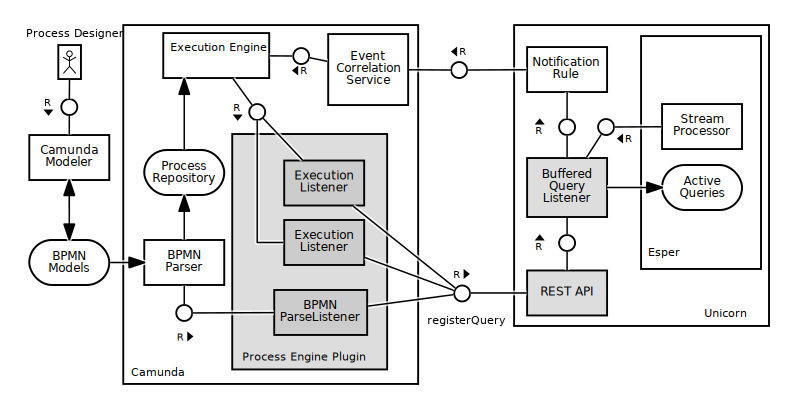
\includegraphics[width=1.3\linewidth]{chapters/implementation/flexible-evt-subscr-camunda-unicorn.png}}
	\caption{Architecture for flexible event subscription in Camunda and Unicorn}
	\label{fig:architecture-camunda-unicorn}
\end{figure}

\section{Extending the Event Processing Platform Unicorn}\label{ch:implunicorn}
\textit{UNICORN} is an event engine developed for academic purposes at the Business Process Technology chair of Hasso-Plattner-Institute, Potsdam.
\cite{herzberg2013event}
It focuses on event processing for \acs{BPM}, ...
Based on Esper, that means, what is esper
what unicorn adds to esper: graphical and rest user-interface to ..., event persistence store, bp execution and correlation, recently also an event generator/replayer
==> it translated user interactions into the according Esper method calls

- currently unicorn uses version 5.3.0 of esper, therefor all future considerations are made based on the documentation of that version

It has been decided to extend the event engine in this scenario, for several reasons.
Firstly, the performance and operation of the process engine shall not be jeopardized. Event Processing features potentially require a lot of performance to handle a large number of requests in a short amount of time.
By implementing the event Buffering module loosely coupled to the Process Engine, we ensure that its performance is not influenced.
Implementing a separate middleware was avoided in the course of this work, to keep the architecture easy and concise to describe.
Unicorn is an academic prototype in constant development and therefor predestined to be directly extended for this kind of use-case.
Moreover, the chosen architecture promises performance advantages thanks to running the event buffering in the same \acs{JVM} as Esper.


\subsection{Event Buffering}
To allow the delayed delivery of events, buffering functionality is added to Unicorn.
Whereas, originally, events that match a certain query in esper are directly forwarded to the notification-recipients, they will instead be held in a buffer until requested by recipient. 
If a recipient is already subscribed, than the behavior will be equivalent to the original scenario, because the event will be delivered instantly.

\paragraph{Engine-specific Implementation Options}
When investigating the options for implementing event buffers in UNICORN, solutions that are specific to the event processing platform were considered.
Notably, the concept of a \textit{Window} in event processing languages is very much comparable with a buffer as described in this work. Windows hold a variable number of events in memory according to specified window properties. That way, windows can act like size- or time-oriented buffers and allow access to older events whenever a new event occurs.
\textit{Named Windows} in Esper allow to create global data windows that can be modified and read from multiple statements. Similar functionality is provided by \textit{Tables}, which follow a relational approach by primary key.
\footnote{see \textit{Chapter 6. EPL Reference: Named Windows And Tables},\newline \url{http://www.espertech.com/esper/release-5.3.0/esper-reference/html/nwtable.html}}

If a query window is connected with the Esper-specific \textit{Output Clause}, it is possible to delay query output with timing constraints or trigger it on the change of a global variable.
\footnote{see \textit{Chapter 5. EPL Reference: Clauses},\newline \url{http://www.espertech.com/esper/release-5.3.0/esper-reference/html/epl\_clauses.html}}
When putting together these features, an event buffer could be implemented as follows: The call \textit{registerQuery} instantiates the window. If the \textit{Consume}-policy is used, we use a named window that we share among queries and delete from after receiving the event. 
At \textit{subscribe}, a notification-recipient is added to a query and output is triggered by causing a variable change in Esper. \textit{Unsubscribe} and \textit{removeQuery} remove a notification-recipient and de-register the query respectively.

A major drawback of this approach is, that the event queries have to be adopted to use the specific features which makes additional knowledge necessary when designing the processes.
Alternatively, the original queries submitted by the process engine can be transformed before registering them in Unicorn, for example by encapsulating them in a sub-query. That way they make use of the mentioned features, but certain expressions will not be possible anymore due to limitations of the Esper EPL with regards to sub-queries.

Apart from this approach, it is worth noting that Unicorn offers a persistent storage of historic events, which can theoretically be used to implement the buffering functionality.
However it would be necessary to abuse the relational approach to implement a persistent stream buffer on top of the SQL database, which is not desirable.

\paragraph{The Generic Buffering Solution}
After considering ... 
none of them is really good
it has been decided to provide a generic buffer implementation that could be applied to any event engine.

we therefor implement three new classes:

How the buffer itself is implemented
+ maintenance module to cope with lifetime policy

it can handle the policies...
(buffered-)QueryListener

the implementation is not trimmed for performance, no shared buffers, maybe ref shared windows from cep
in a production use-case it might be preferable to use the existing technology that the event engine offers if it suits with the requirements of the BPM architecture

\subsection{REST API Extension}
UNICORN offers a restful http api
by default it has the following functionality
section xy demands that the functionality is extended.
the methods are implemented as follows
>
>
>
>
backwards compatibility? do we change the existing calls directly or du we create a new endpoint / new paths?


after implementing the necessary extensions to the event engine, it is the task of the process engine to connect the extended process model to the buffered event handling.
The adaptations to the process engine are presented in the following section.

\section{Event Subscription Handling in Camunda}\label{ch:implcamunda}
through the bpmn extension for flexible event subscription, the information necessary to register event queries in a cep platorm is available in the bpmn model.
\autoref{} outlines how the business process engine must be adapted to execute the operations for subscription handling.
Camunda is an open-source business process engine with support for the latest version of the BPMN. Further information is provided in \autoref{}

\autoref{} depicts the architecure of Camunda, highlighting the modified parts in gray.
for our purposes we consider the core components execution engine, model repository, correlation serviceand the modeler
the tasks of them are...

\subsection{Employing ExecutionListeners in a Process Engine Plugin}
the platform is designed to offer customizability (source)
a core concept to execute own code during process execution are Execution Listeners.
they can be inserted straight into a bpmn model using the camunda modeler as demonstrated in \autoref{assessment}
one of the main goals of introducing the bpmn extension is to get rid of the necessity to explicitly model the subscription in the process (unless an explicit subscription task shall be used).
instead subscriptions shall be managed automatically by the process engine, solely based on the modeled attributes.

To achieve this kind of behavior, Camunda offers the concept of a \ac{PEP} to register global execution listeners.
The plugin is a seperate software module that implements the ... interface. (ref)
it is activated by adding an entry ... in the process engine config.
within the implementation of the plugin, it is possible to intercept the process engine execution at predefined points.
the engine itself implements an event-oriented architecture: significant milestones during engine executions fire an event that execution listeners can react on.
Some of the available events are...

\cite{mandal:2017} and \cite{Pufahl2017} have chosen to directly adapt the source code of camunda. more precisely, they propose to modify the Behavior class to execute additional code when a BPMN element starts executing.
In this work, we implement a Process Engine Plugin as it allows a clearer, more understandable approach to adopting the execution behavior. especially when it is only necessary to execute additional operations and not modify or delete existing code.
the PEP furthermore facilitates re-usability across environments and different versions of Camunda.

..ref illustrates how a pep can be used to execute a piece of code on process instantiation.

A helpful example for using a BPMN Parse Listener is also provided on GitHub\footnote{pep example https://github.com/camunda/camunda-bpm-examples/tree/master/process-engine-plugin/bpmn-parse-listener}.

\missingfigure{chunk of code that shows the main plugin class, how an execution listener is added. and that execution listener does a s.o.p.}

% interface def https://docs.camunda.org/javadoc/camunda-bpm-platform/7.7/?org/camunda/bpm/engine/impl/cfg/ProcessEnginePlugin.html
% peps https://docs.camunda.org/manual/7.7/user-guide/process-engine/process-engine-plugins/


from \autoref{ch:bpmnx:basic}
\todo[inline]{that means that in the implementation we need additional configuration values -> implementation chapter}
%- PEP config properties: cep url

\subsection{Managing event Subscriptions at Runtime}
The Process Engine Plugin enables us to execute custom java code during process deployment, instantiation and execution.
By this means, event subscription and un-subscription can be implemented.

Before event subscription and un-subscription itself can be addressed, it must be ensured that the subscription information is read from the bpmn model.
when a process gets deployed in Camunda, the BPMN-file is read and stored in an internal Java-Object representation.
% read a model https://docs.camunda.org/manual/7.7/user-guide/model-api/bpmn-model-api/read-a-model/
% bpmn extension elements https://docs.camunda.org/manual/7.7/user-guide/model-api/bpmn-model-api/extension-elements/
Custom BPMN extension elements can be accessesd using an in-built generic XML model API.
It allows to read and modify any element in the XML model read from file. The API-call to read the CEP query from the BPMN model is shown in ..ref

\missingfigure{xml model api call to read the cep query and s.o.p. it }

- event correlation
> SubscriptionManager: memorize the subscriptionIDs for a process instance
\cleardoublepage%************************************************
\chapter{Related Work}\label{ch:relatedwork}
%************************************************
% start broad, become narrower, explain differences

% luckham2011event: Event processing for business: organizing the real-time enterprise

The field of \acf{EdBPM} has developed from connecting \ac{CEP} and \ac{BPM} in an attempt to increase the quality and performance of business processes~\cite{luckham2008power} and is an active field of research.
The discipline is investigated from different perspectives.
In event-driven business process monitoring and business activity monitoring, the process engine takes the role of an event producer that publishes information about its process executions to an event engine \cite{baumgrass2014bpmn, herzberg2013improving, bulow2013monitoring}. 
This information can be used to detect process violations, evaluate execution performance and derive key performance indicators during process exeuction \cite{janiesch2011blueprint, janiesch:poc-eventdriven-bam}, whereas the field of process mining intends to derive process knowledge from historic processes~\cite{tiwari2008review}.
In their comprehensive survey on \ac{EdBPM}~\cite{Krumeich2014EventDrivenBP}, Krumeich et. al. distinguish a application possibility, \acf{EdBPC}, where process executions consume events to control the execution flow~\cite{Cabanillas2014, Baumgrass2016}.
An example application is shown by Estruch et. al. \cite{estruch2012event} who incorporate event in a manufacturing process in order to increase process performance.
Pufahl \cite{Pufahl2017} presents a more generic application of business process control in her work on the re-evaluation of decisions based on events.

\cite{chandy2010event} highlights that EdBPC requires an appropriate integration of the CEP component into the control of the business processes.
an essential aspect is subscription and unsubscr. \cite{luckham2008power}

\cite{Cabanillas2014}: investigations on the connection between events and process models, leading to \cite{Baumgrass2016}: extension of bpmn for receiving events, process variables in the query
\cite{Pufahl2017} makes use of events to control process executions and considers event subscription as an essential step in the process. However, the subscription time cannot be chosen flexibly.

\cite{decker2008instantiation}: Process Instantiation, talks a lot about subscription, but no flexible subscr time, nobuffer, only for instantiation
- maybe ref Barros, A., Decker, G., Grosskopf, A.: Complex events in business processes. In: Business Information Systems. Springer (2007), for example in pub/sub principle > temporal order (like mandal et al)


\cite{von2010integrating}: Integrating Complex Events for Collaborating and Dynamically Changing Business Processes; talk about un/subscription, extend ws-bpel with subscription, reporting, patterns, expression language, ..; scope, time of subscription and event buffering not discussed
also: \cite{juric2010wsdl}






%Control the flow: How to safely compose streaming services into business processes
%Modeling and Execution of Event Stream Processing in Business Processes
\cite{appel2014modeling}: includes the streams and stream processing right into the process model
same: \cite{biornstad2006control}


\cite{mandal:2017} has been the starting point for this thesis, not only acknowledging the discrepancy between the event occurrence time in the real world and the event subscription time as interpreted from the BPMN standard, but also incorporating event subscription in the BPMN model.
Inspired by their work, this thesis revisits the topic from scratch
however: ...



- to enable flexible event subscription in bpmn models, we have presented a bpmn extension in accordance with the in-built bpmn extension mechanism
> BPMN extension mechanisms: braun2014classification (most of the extensions are not model conform), braun2015behind (implicit and explicit extension)
> Krumeich2014EventDrivenBP: In most cases these contributions propose an extension of the Business Process Modeling, for modeling goals, high-level events or even whole business situations; p.12 sec 4.1.6



%> predictive: Schwegmann, B., Matzner, M. and Janiesch, C. (2013a), “A method and tool for predictive event-driven process analytics”, in Alt, R. and Franczyk, B. (Eds), Proceedings of the 11th International Conference on Wirtschaftsinformatik (WI2013), Universita¨ t Leipzig, Leipzig, pp. 721-735.


- in this thesis, the queries must be formulated in complete epl. some related work argues that this is too difficult.
\cite{Kunz2010}: acknowledge the lack of usability in CEP and address it by applying bpmn as graphical support for the definition of cep patterns
\cite{gabriel2016konzeptionelle}: generate queries from new graphical notation, anbieterunabhängige Modellierung von EdBPM
- in monitoring this can be derived from the model:
\cite{backmann2013model}: support the automated creation of CEP queries for process MONITORING 
> an automatic generation of queries was also considered in  \cite{Pufahl2017}

- maybe: persisting events in cep platforms | or delayed delivery of events | 
to implement a flexible event subscription time, is has been noted that a temporary storage is required. Seen from the time of consumption, historic events are consumed.

> \cite{roth2010event}: Event data warehousing for complex event processing and \cite{buchmann2010event}:Event-Driven services: Integrating production, logistics and transportation
also \cite{li2007historic}: historic data in pub/sub
> but if i want to have that historic information, than I would have to issue a subscription some time before. I integrate everything in the process model

- event buffering for the application in a BPM environment may not be confused with internal buffering techniques used within event engines to perform load shedding, even out short term load peaks. 
%see https://books.google.de/books?id=MWCfC9OKaToC&pg=PA198&lpg=PA198&dq=event+processing+optimization+overlapping+windows&source=bl&ots=yfcNb0YGAg&sig=qrYgyfRV-bLesOcCyxpeBdCQTr0&hl=de&sa=X&ved=0ahUKEwit2czXytbVAhVCD5oKHWdYAGAQ6AEIPjAC#v=onepage&q=event%20processing%20optimization%20overlapping%20windows&f=false
% Stream Data Processing: A Quality of Service Perspective: Modeling von Sharma Chakravarthy,Jiang Qingchun, 9.3.6


\cleardoublepage%************************************************
\chapter{Conclusion}\label{ch:conclusion}
%************************************************

% what general topic was addressed and why
As organizations have adopted comprehensive business process management solutions, they are constantly seeking to improve process capabilities, quality and performance.
Integrating Complex Event Processing into their business workflows is a popular means to increase process flexibility.
As event-driven architectures mostly operate according to the publish-subscribe paradigm, the support of this interaction pattern is increasingly important when modeling business processes.
The industry-standard \acf{BPMN} offers comprehensive support for events but does not address subscribe-operations specifically.
The common understanding is that the subscription to an event only takes place when it gets enabled, so that events that occur before cannot be consumed.

% what has been done
Motivated by the possible process execution issues implied by the bad BPMN specification, this work has investigated the topic of event subscription in bpmn.
Initially, the motivating scenarios and related work has been translated into three requirements R1-R3 that a business process meta model must fulfill to address the previously stated problems.
The core of these requirements is that there must be a possibility to influence the event subscription time, including subscription times before process instantiation and deployment. 
The choice of event subscription times takes into consideration the event occurrence scenarios.
Apart from that it was stated that the event subscription time must be explicit in the model to address the lack of specification in the BPMN model
Given that event subscription and consumption are not performed at the same time, the need for a temporary storage of events was identified.

%assessment
In the following chapter REF we have investigated for each requirement, to what extent it can be expressed in the BPMN.
For most of the aspects, it was possible to find acceptable solutions, though the complexity of the models did increase in every case.
This became especially apparent when analyzing the event occurrence scenarios before instantiation and before deployment. A complex business process model involving two additional auxiliary processes was presented to enable event subscription and event buffering in these cases.
An implementation of the processes using the Camunda business process engine was presented.
%By implementing the flexible event subscription concept in Unicorn and Camunda it could be demonstrated that state-of-the-art BPM and CEP technology is flexible enough to handle ..., but
The results of that analysis where summarized in three shortcomings, S1-S3, complaining about the increase in model complexity, about the mis-use of BPMN for infrastructure tasks and about the possible performance limitations when implementing flexible subscription and event buffering in bpmn.

%concept
Together, the requirements and the shortcomings were taken as a foundation to develop a BPMN extension that allows an explicit and flexible use of event subscription in business process.
The extension builds upon the addition of subscription-related information to the BPMN Message type. it requires that all information necessary to issue a subscription can be obtained from the model.
The extension aims to offer a convenient use of subscription operations by automatizing the subscription operations in the process engine.
As the execution semantics of bpmn intermediate events and the receive task are extended with automatic subscription handling, there are additional requirements to the process engine and to the event processing platform, which are outlined as part of the extension.

%implementation
Given the model extension and the derived requirements to process engine and event processing API, Chapter XX describes a reference implementation at the example of Camunda and the event processing platform Unicorn.
Camunda has been extended with subscription handling functionality, issuing event subscription and un-subscription in accordance with the extended process models.
Therefor, a process engine plugin was implemented around a central ParseListener that injects custom code when a business process model is deployed and a number of ExecutionListeners that can control subscription and un-subscription during the execution of the process.
Thanks to the plugin-mechanism, the resulting artifact is easily portable and can be used across different versions of the process engine.
To add the necessary functionality to Unicorn, its code-base has been extended with an event buffering module and additional webservice API calls.
Combined, the two are able to process and execute process models using the newly introduced bpmn extension for flexible event subscription

%conclusions
The results of this thesis provide a comprehensive study of event subscription mechanisms business processes. 
The investigations have led to a bpmn extension to express subscription semantics in bpmn models and an according implementation to evaluate the results.

% what were the limitations of this thesis and what can be done in the future


\section{Discussion}

- discussion:
> it remains the problem, that epl knowledge is not available in process design, a problem that has been addressed in ...
> while the event buffering can now be controlled from the process model level, events must still be acquired by the event engine before (set up event types and make sure that the events are pushed to the engine)
> the concept tries to bridge the gap between event persistence/historic events and real-time event processing by arguing that event occurrences are kept for a limited time and can therefor still be treated as events. A contra argumentation might be that an event becomes a simple piece of information as soon as it is not instantaneously consumed. hence it should not be modeled as an event but simply as a data object, using a data store
> many design decisions have been begründet with an improved usability though no empirical basis was available. Reasoning was only based on literature and chats with a small group of fellow researchers

- it can be argued that at process design time you dont care about the subscription time itself, but about the maximum age you can accept for your events. this would connect the lifetimepolicy and the subscription time into one value. but make the processing more complex and more fuzzy

\section{Future Work}

- modeling subscription dependencies as data objects and automatically evaluating the earliest possible time of subscription
- (Andreas:) using the bpmn extension with multiple event engines
- this work attempts to provide a standard for handling event subscription in bpm architectures. given the necessity and the repeated attempts to address to topic, it would be a reasonable next step to discuss available solutions and start providing a foundation that is accepted and reused across the bpm community. No matter if based on the solutions of this work or not.
> it must be evaluated if that's the way event buffering shall be used. > prove the value of flexible event subscription in an industry case study
- future work: event data from other events could be used as historic data to allow the access even before process deployment
- time of subscription could also be defined as "at termination of activity xy"
- visual representation of the extended meta-model
- formal execution semantics to allow/facilitate automatized model-checking


%\addtocontents{toc}{\protect\clearpage} % <--- just debug stuff, ignore
%\include{multiToC} % <--- just debug stuff, ignore for your documents
% ********************************************************************
% Backmatter
%*******************************************************
\appendix
%\renewcommand{\thechapter}{\alph{chapter}}
\cleardoublepage
%************************************************
\chapter{Appendix}
%************************************************

\begin{lstlisting}[basicstyle=\scriptsize,caption={XSD schema of the BPMN extension for flexible event subscription},label=lst:xsd-flexsub]
<xsd:schema xmlns:flexsub="http://www.some.url/" xmlns:xsd="http://www.w3.org/2001/XMLSchema" targetNamespace="http://www.some.url/">
<xsd:element name="eventSubscriptionTask" type="tEventSubscriptionTask" />
<xsd:complexType name="tEventSubscriptionTask">
<xsd:complexContent>
<xsd:extension base="tTask">
<xsd:attribute name="messageId" type="xsd:QName" use="required"/>
</xsd:extension>
</xsd:complexContent>
</xsd:complexType>

<xsd:element name="subscriptionDefinition">
<xsd:complexType>
<xsd:sequence>
<xsd:element type="xsd:string" name="eventQuery" minOccurs="1" maxOccurs="1" />
<xsd:element type="tSubscriptionTime" name="subscriptionTime" minOccurs="0" maxOccurs="1" default="Element Execution"/>
<xsd:element name="bufferPolicies" minOccurs="0" maxOccurs="1">
<xsd:complexType>
<xsd:sequence>
<xsd:element type="xsd:string" name="lifespanPolicy" minOccurs="0" maxOccurs="1" default="infinite"/>
<xsd:element type="xsd:string" name="consumptionPolicy" minOccurs="0" maxOccurs="1" default="Reuse"/>
<xsd:element type="xsd:integer" name="sizePolicy" minOccurs="0" maxOccurs="1" default="0"/>
<xsd:element type="tOrderPolicy" name="orderPolicy" minOccurs="0" maxOccurs="1" default="FIFO"/>
</xsd:sequence>
</xsd:complexType>
</xsd:element>
</xsd:sequence>
</xsd:complexType>
</xsd:element>

<xsd:simpleType name="tSubscriptionTime">
<xsd:restriction base="xsd:string">
<xsd:enumeration value="Process Deployment"/>
<xsd:enumeration value="Process Instantiation"/>
<xsd:enumeration value="Manual"/>
<xsd:enumeration value="Element Execution"/>
</xsd:restriction>
</xsd:simpleType>

<xsd:simpleType name="tOrderPolicy">
<xsd:restriction base="xsd:string">
<xsd:enumeration value="LIFO"/>
<xsd:enumeration value="FIFO"/>
</xsd:restriction>
</xsd:simpleType>
</xsd:schema>
\end{lstlisting}

\todo[inline]{complete xml example of a BPMN model using the extensions}


%********************************************************************
% Other Stuff in the Back
%*******************************************************
\cleardoublepage\include{frontbackmatter/Bibliography}
\cleardoublepage%*******************************************************
% Declaration
%*******************************************************
\refstepcounter{dummy}
\pdfbookmark[0]{Declaration}{declaration}
\chapter*{Eigenständigkeitserklärung}
\thispagestyle{empty}

Hiermit erkäre ich an Eides statt, dass:

\begin{itemize}
	\item wörtlich aus anderer Quelle übernommene Teile der Arbeit deutlich
	als Zitat gekennzeichnet sind und mit Quellenangabe versehen
	sind;
	
	\item sinngemäß aus anderen Quellen übernommene Teile der Arbeit
	mit Quellenangabe versehen sind;
	
	\item alle übrigen Teile der Arbeit von mir ohne inhaltliche oder wörtliche
	Übernahme von Teilen anderer Werke erarbeitet sind.
	
\end{itemize}

\bigskip
 
\noindent\textit{\myLocation, \myTime}

\smallskip

\begin{flushright}
    \begin{tabular}{m{5cm}}
        \\ \hline
        \centering\myName \\
    \end{tabular}
\end{flushright}

\cleardoublepage\include{frontbackmatter/Colophon}
% ********************************************************************
% Game Over: Restore, Restart, or Quit?
%*******************************************************
\end{document}
% ********************************************************************
